\cchapter{Loop Transformations}{loop_transformations}
\label{chap:loop_transformations}

To obtain better performance on a platform, code may need to be restructured 
relative to the way it is written (which is often for best readability).
User-directed loop transformations accomplish this goal by providing a means 
to separate code semantics and its optimization.

A loop transformation construct states that a transformation operation is to be 
performed on set of nested loops.  This directive approach can target specific loops
for transformation, rather than applying more time-consuming general compiler 
heuristics methods with compiler options that may not be able to discover 
optimal transformations.

Loop transformations can be augmented by preprocessor support or OpenMP \kcode{metadirective} 
directives, to select optimal dimension and size parameters for specific platforms,
facilitating a single code base for multiple platforms.
Moreover, directive-based transformations make experimenting easier: 
whereby specific hot spots can be affected by transformation directives.


%===== Examples Sections =====
%\pagebreak
\section{\code{tile} Construct}
\label{sec:tile}
\index{constructs!tile@\code{tile}}
\index{tile construct@\code{tile} construct}
\index{tile construct@\code{tile} construct!sizes clause@\code{sizes} clause}
\index{sizes clause@\code{sizes} clause}
\index{clauses!sizes@\code{sizes}}

In the following example a \code{tile} construct transforms two nested loops
within the \texttt{func1} function into four nested loops.
The tile sizes in the \code{sizes} clause are applied from outermost
to innermost loops (left-to-right). The effective tiling operation is illustrated in
the \texttt{func2} function. 
(For easier illustration, tile sizes for all examples in this section evenly 
divide the iteration counts so that there are no remainders.)

In the following C/C++ code the inner loop traverses columns
and the outer loop traverses the rows of a 100x128 (row x column) matrix.  
The \code{sizes(5,16)} clause of the \code{tile} construct specifies
a 5x16 blocking, applied to the outer (row) and inner (column) loops.
The worksharing-loop construct before the \code{tile}
construct is applied after the transform.

\cexample[5.1]{tile}{1}

In the following Fortran code the inner loop traverses rows 
and the outer loop traverses the columns of a 128x100 (row x column) matrix.  
The  \code{sizes(5,16)} clause of the \code{tile} construct specifies 
a 5x16 blocking, applied to the outer (column) and inner (row) loops.
The worksharing-loop construct before the \code{tile}
construct is applied after the transform.

\ffreeexample[5.1]{tile}{1}
\clearpage

This example illustrates transformation nesting.
Here, a 4x4 ``outer''  \code{tile} construct is applied to the ``inner'' tile transform shown in the example above.
The effect of the inner loop is shown in \texttt{func2} (cf.\ \texttt{func2} in tile.1.c).
The outer \code{tile} construct's \code{sizes(4,4)} clause applies a 4x4 tile upon the resulting
blocks of the inner transform.  The effective looping is shown in \texttt{func3}.

\cexample[5.1]{tile}{2}
\ffreeexample[5.1]{tile}{2}

\pagebreak
\section{Incomplete Tiles}
\label{sec:incomplete_tiles}

Optimal performance for tiled loops is achieved when the loop iteration count is a multiple of the tile size.
When this condition does not exist, the implementation is free to execute the partial loops in a manner that
optimizes performance, while preserving the specified order of iterations in the complete-tile loops.

Figure~\ref{fig:2d_tiling} shows an example of a 2-by-2 tiling for a 5-by-5 iteration space.
There are nine resulting tiles. Four are \emph{complete} 2-by-2 tiles, and the
remaining five tiles are \plc{partial} tiles.

\begin{figure}[H]
\begin{subfigure}[b]{.5\textwidth}
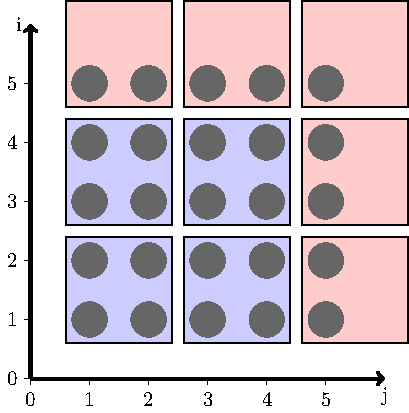
\includegraphics[width=0.8\textwidth]{figs/tile-2d_tiling}
\centering
\caption{2-dimensional tiling with partial tiles}\label{fig:2d_tiling}
\end{subfigure}%
\begin{subfigure}[b]{.5\textwidth}
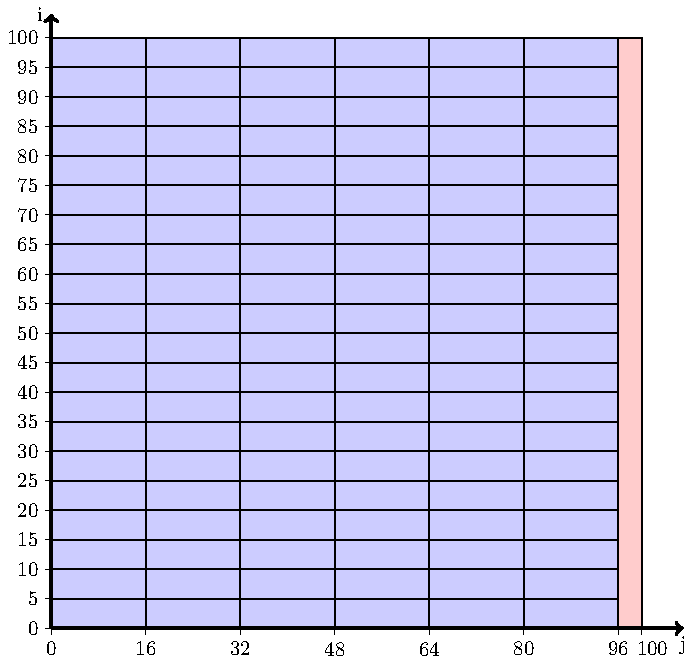
\includegraphics[width=0.85\textwidth]{figs/tile-Example_tile2}
\vspace*{2mm}
\centering
\caption{Partial tiles of Example \emph{partial\_tile.1}}\label{fig:Example_tile2}
\end{subfigure}
\caption{Tiling illustrations}
\end{figure}

In the following example, function \plc{func1} uses the \code{tile} construct
with a \code{sizes(4,16)} tiling clause.  Because the second tile dimension of
16 does not evenly divide into the iteration count of the j-loop, the
iterations corresponding to the remainder for the j-loop correspond to partial
tiles as shown in Figure~\ref{fig:Example_tile2}. Each remaining function
illustrates a code implementation that a compiler may generate to implement the
\code{tile} construct in \plc{func1}.

%Iterations with the tiles can be executed in a any order, ignoring partial tile boundaries.
% Deepak: I don't think this first sentence is true for iterations in a partial tile.
% Only the product order will be maintained for such iterations.
The order of tile execution relative to other tiles can be changed, but execution order of 
iterations within the same tile must be preserved.
Implementations must ensure that dependencies that are valid with any tile size need
to be preserved (including tile size of 1 and tiles as large as the iteration space).

Functions \plc{func2} through \plc{func6} are valid implementations of \plc{func1}.
In \splc{func2} the unrolling is illustrated as a pair of nested loops with a simple
adjustment in the size of the final iteration block in the \splc{j2} iteration space
for the partial tile.

Performance of the implementation depends on the hardware architecture, the instruction set and compiler optimization goals.
Functions \plc{func3}, \plc{func4}, and  \plc{func5} have the advantage that
the innermost loop for the complete tile is a constant size and can be replaced with SIMD instructions.
If the target platform has masked SIMD instructions with no overhead, then avoiding the construction of a
remainder loop, as in \plc{func5}, might be the best option.
Another option is to use a remainder loop without tiling, as shown in \plc{func6}, to reduce control-flow overhead.

\cexample[5.1]{partial_tile}{1}
\ffreeexample[5.1]{partial_tile}{1}


In the following example, function \plc{func7} tiles nested loops with a size of (4,16),
resulting in partial tiles that cover the last 4 iterations of the j-loop, as
in the previous example.  However, the outer loop is parallelized with a
\code{parallel} worksharing-loop construct.

Functions \plc{func8} and \plc{func9} illustrate two implementations of the tiling
with \code{parallel} and worksharing-loop directives.  Function \plc{func8} uses a single outer loop, with a \plc{min} function
to accommodate the partial tiles. Function \plc{func9}
uses two sets of nested loops, the first iterates over the complete tiles and the
second covers iterations from the partial tiles. When fissioning loops that
are in a \code{parallel} worksharing-loop region, each iteration of each workshared loop
must be executed on the same thread as in an un-fissioned loop.  The \code{schedule(static)} clause in \plc{func7}
forces the implementation to use static scheduling and allows the fission in function \plc{func8}.
When dynamic scheduling is prescribed, fissioning is not allowed.  When no scheduling is specified,
the compiler implementation will select a scheduling \plc{kind} and adhere to its restrictions.

\cexample[5.1]{partial_tile}{2}
\ffreeexample[5.1]{partial_tile}{2}

\pagebreak
\section{\kcode{unroll} Construct}
\label{sec:unroll}
\index{constructs!unroll@\kcode{unroll}}
\index{unroll construct@\kcode{unroll} construct}
\index{unroll construct@\kcode{unroll} construct!full clause@\kcode{full} clause}
\index{full clause@\kcode{full} clause}
\index{clauses!full@\kcode{full}}
\index{unroll construct@\kcode{unroll} construct!partial clause@\kcode{partial} clause}
\index{partial clause@\kcode{partial} clause}
\index{clauses!partial@\kcode{partial}}

The \kcode{unroll} construct is a loop transformation that increases the 
number of loop blocks in a loop, while reducing the number of iterations.
The \kcode{full} clause specifies that the loop is to be completely unrolled.  
That is, a loop block for each iteration is created, and the loop is removed.
A \kcode{partial} clause  with an \plc{unroll-factor} specifies that the number of
iterations will be reduced multiplicatively by the factor while the number of 
blocks will be increased by the same factor.  
Operationally, the loop is tiled by the factor, and the tiled loop is 
fully expanded, resulting in a single loop with multiple blocks.

Unrolling can reduce control-flow overhead and provide additional
optimization opportunities for the compiler and the processor
pipeline. Nevertheless, unrolling can increase the code size, and saturate
the instruction cache. Hence, the trade-off may need to be assessed.
Unrolling a loop does not change the code's semantics. Also, compilers
may unroll loops without explicit directives, at various optimization levels.

In the example below, the \kcode{unroll} construct is used without any clause, and then
with a \kcode{full} clause, in the first two functions, respectively.
When no clause is used, it is up to the implementation (compiler) 
to decide if and how the loop is to be unrolled.  
The iteration count can have a run time value.  
In the second function, the \kcode{unroll} construct uses a \kcode{full} clause
to completely unroll the loop.  A compile-time constant is required for the iteration count.
The statements in the third function (\ucode{unroll_full_equivalent}) illustrates
equivalent code for the full unrolling in the second function.

\cexample[5.1]{unroll}{1}
\ffreeexample[5.1]{unroll}{1}


The next example shows cases when it is incorrect to use full unrolling.

\cexample[5.1]{unroll}{2}
\ffreeexample[5.1]{unroll}{2}

In many cases, when the iteration count is large and/or dynamic, it is
reasonable to partially unroll a loop by including a \kcode{partial} clause.
In the \ucode{unroll3_partial} function below, the \plc{unroll-factor} value
of 4 is used to create a tile size of 4 that is unrolled to create 4 unrolled statements.
The equivalent ``hand unrolled'' loop code is presented in the 
\ucode{unroll3_partial_equivalent} function.
If the \plc{unroll-factor} is omitted, as in the \ucode{unroll3_partial_nofactor} 
function, the implementation may optimally select a factor from 1 
(no unrolling) to the iteration count (full unrolling).  
In the latter case the construct generates a loop with a single iteration.

\cexample[5.1]{unroll}{3}
\ffreeexample[5.1]{unroll}{3}

When the iteration count is not a multiple of the \plc{unroll-factor},
iterations that should not produce executions must be conditionally
protected from execution. In this example, the first function
unrolls a loop that has a variable iteration count. Since the \kcode{unroll}
construct uses a \kcode{partial(\ucode{4})} clause, the compiler will need to
create code that can account for cases when the iteration count is not a
multiple of 4. A brute-force, simple-to-understand approach for implementing 
the conditionals is shown in the \ucode{unroll_partial_remainder_option1} function.

The remaining two functions show more optimal algorithms the compiler 
may select to implement the transformation.
Optimal approaches may reduce the number of conditionals as shown in 
\ucode{unroll_partial_remainder_option2}, and 
may eliminate conditionals completely by peeling off a ``remainder'' 
into a separate loop as in \ucode{unroll_partial_remainder_option3}. 

Regardless of the optimization, implementations must ensure that the semantics
remain the same, especially when additional directives are applied to
the unrolled loop. For the case in the \ucode{unroll_partial_remainder_option3}
function, the fission of the worksharing-loop construct may result in a different
distribution of threads to the iterations. Since no reproducible scheduling
is specified on the work-sharing construct, the worksharing-loop and unrolling are compliant.

\cexample[5.1]{unroll}{4}
\ffreeexample[5.1]{unroll}{4}

\pagebreak
\section{\kcode{apply} Clause}
\label{sec:apply_clause}

\index{unroll construct@\kcode{unroll} construct!apply clause@\kcode{apply} clause}
\index{tile construct@\kcode{tile} construct!apply clause@\kcode{apply} clause}

\index{apply clause@\kcode{apply} clause}
\index{clauses!apply@\kcode{apply}}

A loop transformation construct can be applied to another nested
loop transformation construct, but the application of the ``outer'' transformation
is limited to the outermost generated loop of the ``inner'' transformation.

The \kcode{apply} clause on a loop transformation construct can specify additional
loop transformation directives that apply to generated loops other than the outermost one.
Clause modifiers are used to specify which generated loop to target.
Also, an applied directive within a clause may specify another \kcode{apply} clause.

%The \code{apply} clause on a loop transformation construct can specify (other)
%loop transformation directives to be applied to its transformation.
%Clause modifiers can be used to target specific generated loops, providing a mechanism
%to overcome the restriction of applying a transformation immediately to the next loop
%transformation construct. Also, an applied directive within a clause may be another
%\code{apply} clause.

Any nested loop transformation constructs including any constructs that
result from \kcode{apply} clauses of nested constructs are replaced before any enclosing
loop transformation construct. This is referred to as the \plc{innermost-first order}
here.

\subsection{Syntax and Effect}

In the example below, the \ucode{construct_unroll} and \ucode{apply_unroll} functions
illustrate the syntax for two equivalent means of applying the \kcode{unroll} loop transformation
directive to the outermost generated (grid) loop of the \kcode{tile} construct transformation.
In function \ucode{construct_unroll}, the tile transformation creates the generated (tiled) loops
and then the \kcode{unroll} construct is applied to outermost loop of the replacement.
In the \ucode{apply_unroll} function, the \kcode{apply} clause on the \kcode{tile} construct
is used to apply an \kcode{unroll} transformation on the \plc{grid} loop (the outermost loop
of the tile transformation) as specified by the \kcode{grid} modifier.

\cexample[6.0]{apply_syntax}{1}
\ffreeexample[6.0]{apply_syntax}{1}

For the two functions in the previous example,
the \ucode{equivalent} function in the next example shows an equivalent
code that a user could have written without using the \kcode{tile} construct
or \kcode{apply} clause.

\cexample[5.1]{apply_syntax_equivalent}{1}
\ffreeexample[5.1]{apply_syntax_equivalent}{1}


The following example shows how multiple loop transformation directives
can be applied to different generated loops resulting from a loop transformation.
For the 4x4 \kcode{tile} construct there will be two (outer) \plc{grid} loops and two (inner) \plc{intra-tile} loops.
The first \kcode{apply} clause specifies that the two \plc{grid} loops are to have an \kcode{interchange} directive and a \kcode{nothing} directive
(just a placeholder to indicate no directive application) applied to the grid (two outermost) loops.
Directives, read from left to right, are applied to the \plc{grid} loops, from outermost to innermost, respectively.
The second \kcode{apply} clause specifies that the two \plc{intratile} loops are to have \kcode{nothing} and \kcode{interchange} directives applied to the
last two \plc{tile} loops, respectively.
Note that the \ucode{A} array dimensions are \ucode{A[100][100][3]} and \ucode{A(0:2,0:99,0:99)}
in the C/C++ and Fortran codes to illustrate equivalent sequential memory access for the
\ucode{i}, \ucode{j} and \ucode{k} loops.

\index{interchange directive@\kcode{interchange} directive}
\index{directives!interchange@\kcode{interchange}}
\index{nothing directive@\kcode{nothing} directive}
\index{directives!nothing@\kcode{nothing}}

\cexample[6.0]{apply_syntax}{2}
\pagebreak
\ffreeexample[6.0]{apply_syntax}{2}

For the function in the previous example,
the \ucode{equivalent} function in the next example shows a possible
equivalent tile replacement code (\kcode{tile} generated loops) and the
appropriately positioned \kcode{interchange} and \kcode{nothing} directives.

\cexample[6.0]{apply_syntax_equivalent}{2}
\pagebreak
\ffreeexample[6.0]{apply_syntax_equivalent}{2}


\index{tile construct@\kcode{tile} construct!apply clause@\kcode{apply} clause}
\index{grid modifier@\kcode{grid} modifier}
\index{intratile modifier@\kcode{intratile} modifier}

The following example illustrates the use of \kcode{apply} clause 
modifiers with argument. The index of the generated loop instead of
a positional location can be used for the applied-directive. 
The \kcode{grid(1)} modifier indicates the first grid loop 
generated by the \kcode{tile} directive
and the \kcode{intratile(2)} modifier indicates the second tile loop
generated by the \kcode{tile} directive.

\cexample[6.0]{apply_syntax}{3}
\pagebreak
\ffreeexample[6.0]{apply_syntax}{3}

Without the index arguments, the \kcode{nothing} argument would
be needed as a placeholder, as illustrated by the equivalent codes
of the above example as follows.

\cexample[6.0]{apply_syntax_equivalent}{3}
\pagebreak
\ffreeexample[6.0]{apply_syntax_equivalent}{3}


\subsection{Spanning Loop Associations}

It is possible for a loop transformation directive to be applied to multiple generated loops,
and multiple directives applied to the same generated loop.
The latter is illustrated in the this example.

\cexample[6.0]{apply_span}{1}
\ffreeexample[6.0]{apply_span}{1}

In this example, the functions show successive steps in the application of
the previous loop transformation example as equivalent user-written code.
First, the tiling is applied in the \ucode{step1} function.
Next, loop transformations in the generated loop nest are replaced according to the innermost-first order rule.
Applying the innermost transformation, loop reversal, results in the loop nest in \ucode{step2}.
After that, the inner tile directive is applied in the \ucode{step3} function.

\index{reverse directive@\kcode{reverse} directive}
\index{directives!reverse@\kcode{reverse}}

\cexample[6.0]{apply_span_equivalent}{1}
\ffreeexample[6.0]{apply_span_equivalent}{1}


\subsection{Nested apply}

The following example illustrates how multiple loop transformations can be chained by nesting \kcode{apply} clauses.
In the \ucode{nested_apply} function, a loop is first tiled, then the intra-tile
loop is unrolled, and finally the iteration order of the unrolled loop is reversed.
For C/C++ codes, reversing a loop with an unsigned type index may cause the compiler
to ensure that underflow is handled correctly.

\cexample[6.0]{apply_nested}{1}
\ffreeexample[6.0]{apply_nested}{1}

In this example the \ucode{step1}, \ucode{step2} and \ucode{step3}
functions are all equivalent to the \ucode{nested_apply} function, but illustrate
a possible chain of transformations but done manually by a user.

\cexample[6.0]{apply_nested_equivalent}{1}
\ffreeexample[6.0]{apply_nested_equivalent}{1}


